\documentclass[twoside]{book}

% Packages required by doxygen
\usepackage{calc}
\usepackage{doxygen}
\usepackage{graphicx}
\usepackage[utf8]{inputenc}
\usepackage{makeidx}
\usepackage{multicol}
\usepackage{multirow}
\usepackage{textcomp}
\usepackage[table]{xcolor}

% Font selection
\usepackage[T1]{fontenc}
\usepackage{mathptmx}
\usepackage[scaled=.90]{helvet}
\usepackage{courier}
\usepackage{amssymb}
\usepackage{sectsty}
\renewcommand{\familydefault}{\sfdefault}
\allsectionsfont{%
  \fontseries{bc}\selectfont%
  \color{darkgray}%
}
\renewcommand{\DoxyLabelFont}{%
  \fontseries{bc}\selectfont%
  \color{darkgray}%
}

% Page & text layout
\usepackage{geometry}
\geometry{%
  a4paper,%
  top=2.5cm,%
  bottom=2.5cm,%
  left=2.5cm,%
  right=2.5cm%
}
\tolerance=750
\hfuzz=15pt
\hbadness=750
\setlength{\emergencystretch}{15pt}
\setlength{\parindent}{0cm}
\setlength{\parskip}{0.2cm}
\makeatletter
\renewcommand{\paragraph}{%
  \@startsection{paragraph}{4}{0ex}{-1.0ex}{1.0ex}{%
    \normalfont\normalsize\bfseries\SS@parafont%
  }%
}
\renewcommand{\subparagraph}{%
  \@startsection{subparagraph}{5}{0ex}{-1.0ex}{1.0ex}{%
    \normalfont\normalsize\bfseries\SS@subparafont%
  }%
}
\makeatother

% Headers & footers
\usepackage{fancyhdr}
\pagestyle{fancyplain}
\fancyhead[LE]{\fancyplain{}{\bfseries\thepage}}
\fancyhead[CE]{\fancyplain{}{}}
\fancyhead[RE]{\fancyplain{}{\bfseries\leftmark}}
\fancyhead[LO]{\fancyplain{}{\bfseries\rightmark}}
\fancyhead[CO]{\fancyplain{}{}}
\fancyhead[RO]{\fancyplain{}{\bfseries\thepage}}
\fancyfoot[LE]{\fancyplain{}{}}
\fancyfoot[CE]{\fancyplain{}{}}
\fancyfoot[RE]{\fancyplain{}{\bfseries\scriptsize Generated on Thu Apr 27 2017 00\-:44\-:48 for moveittutorials\-\_\-documentation by Doxygen }}
\fancyfoot[LO]{\fancyplain{}{\bfseries\scriptsize Generated on Thu Apr 27 2017 00\-:44\-:48 for moveittutorials\-\_\-documentation by Doxygen }}
\fancyfoot[CO]{\fancyplain{}{}}
\fancyfoot[RO]{\fancyplain{}{}}
\renewcommand{\footrulewidth}{0.4pt}
\renewcommand{\chaptermark}[1]{%
  \markboth{#1}{}%
}
\renewcommand{\sectionmark}[1]{%
  \markright{\thesection\ #1}%
}

% Indices & bibliography
\usepackage{natbib}
\usepackage[titles]{tocloft}
\setcounter{tocdepth}{3}
\setcounter{secnumdepth}{5}
\makeindex

% Custom commands
\newcommand{\clearemptydoublepage}{%
  \newpage{\pagestyle{empty}\cleardoublepage}%
}


%===== C O N T E N T S =====

\begin{document}

% Titlepage & ToC
\pagenumbering{roman}
\begin{titlepage}
\vspace*{7cm}
\begin{center}%
{\Large moveittutorials\-\_\-documentation }\\
\vspace*{1cm}
{\large Generated by Doxygen 1.8.6}\\
\vspace*{0.5cm}
{\small Thu Apr 27 2017 00:44:48}\\
\end{center}
\end{titlepage}
\clearemptydoublepage
\tableofcontents
\clearemptydoublepage
\pagenumbering{arabic}

%--- Begin generated contents ---
\chapter{Move\-It! Tutorials}
\label{md__r_e_a_d_m_e}
This repo is automatically built by the R\-O\-S build farm and its output is hosted here\-: {\tt http\-://docs.\-ros.\-org/indigo/api/moveit\-\_\-tutorials/html/}

\subsection*{Travis Continuous Integration}

{\tt ![Build Status](https\-://travis-\/ci.\-org/ros-\/planning/moveit\-\_\-tutorials.\-svg?branch=master)}

\subsection*{R\-O\-S Buildfarm}

{\tt ![Build Status](http\-://build.\-ros.\-org/build\-Status/icon?job=\-Idoc\-\_\-\-\_\-moveit\-\_\-tutorials\-\_\-\-\_\-ubuntu\-\_\-trusty\-\_\-amd64\&build=2)}

\subsection*{Build}

If you want to test the tutorials by generating the html pages locally on your machine, install {\tt rosdoc\-\_\-lite}\-: \begin{DoxyVerb}sudo apt-get install ros-kinetic-rosdoc-lite
\end{DoxyVerb}


and run in the root of the package\-: \begin{DoxyVerb}rosdoc_lite -o build .
\end{DoxyVerb}


Then open {\ttfamily L\-O\-C\-A\-L\-\_\-\-P\-A\-C\-K\-A\-G\-E\-\_\-\-P\-A\-T\-H/build/html/index.\-html} in your web browser.

\subsection*{Deployment}

For deploying documentation changes to the web, {\tt Section 3 of rosdoc\-\_\-lite wiki} says that \char`\"{}rosdoc\-\_\-lite is automatically run for packages in repositories that have rosinstall files listed in the rosdistro repository.\char`\"{} This is done about once every 24 hours, {\tt overnight}. 
\chapter{Namespace Index}
\section{Namespace List}
Here is a list of all documented namespaces with brief descriptions\-:\begin{DoxyCompactList}
\item\contentsline{section}{{\bf sphinx\-\_\-rtd\-\_\-theme} }{\pageref{namespacesphinx__rtd__theme}}{}
\item\contentsline{section}{{\bf tutorialformatter} }{\pageref{namespacetutorialformatter}}{}
\end{DoxyCompactList}

\chapter{Hierarchical Index}
\section{Class Hierarchy}
This inheritance list is sorted roughly, but not completely, alphabetically\-:\begin{DoxyCompactList}
\item Directive\begin{DoxyCompactList}
\item \contentsline{section}{tutorialformatter.\-Tutorial\-Formatter\-Directive}{\pageref{classtutorialformatter_1_1_tutorial_formatter_directive}}{}
\end{DoxyCompactList}
\item exception\begin{DoxyCompactList}
\item \contentsline{section}{Interactive\-Robot\-:\-:Robot\-Load\-Exception}{\pageref{class_interactive_robot_1_1_robot_load_exception}}{}
\end{DoxyCompactList}
\item \contentsline{section}{I\-Marker}{\pageref{class_i_marker}}{}
\item \contentsline{section}{Interactive\-Robot}{\pageref{class_interactive_robot}}{}
\end{DoxyCompactList}

\chapter{Class Index}
\section{Class List}
Here are the classes, structs, unions and interfaces with brief descriptions\-:\begin{DoxyCompactList}
\item\contentsline{section}{{\bf Check\-Value$<$ T $>$} }{\pageref{struct_check_value}}{}
\item\contentsline{section}{{\bf I\-K\-Solver} }{\pageref{class_i_k_solver}}{}
\end{DoxyCompactList}

\chapter{Namespace Documentation}
\section{sphinx\-\_\-rtd\-\_\-theme Namespace Reference}
\label{namespacesphinx__rtd__theme}\index{sphinx\-\_\-rtd\-\_\-theme@{sphinx\-\_\-rtd\-\_\-theme}}
\subsection*{Functions}
\begin{DoxyCompactItemize}
\item 
def {\bf get\-\_\-html\-\_\-theme\-\_\-path}
\end{DoxyCompactItemize}
\subsection*{Variables}
\begin{DoxyCompactItemize}
\item 
tuple {\bfseries V\-E\-R\-S\-I\-O\-N} = (0, 1, 8)\label{namespacesphinx__rtd__theme_add8d364c7e5520747da57b7c58f01792}

\item 
string {\bfseries \-\_\-\-\_\-version\-\_\-\-\_\-} = \char`\"{}.\char`\"{}\label{namespacesphinx__rtd__theme_a80f76b3669bb1e6addf92ad73f2cc0e5}

\item 
{\bfseries \-\_\-\-\_\-version\-\_\-full\-\_\-\-\_\-} = \-\_\-\-\_\-version\-\_\-\-\_\-\label{namespacesphinx__rtd__theme_ade673d940f4f03941033f9687f249130}

\end{DoxyCompactItemize}


\subsection{Detailed Description}
\begin{DoxyVerb}Sphinx ReadTheDocs theme.

From https://github.com/ryan-roemer/sphinx-bootstrap-theme.\end{DoxyVerb}
 

\subsection{Function Documentation}
\index{sphinx\-\_\-rtd\-\_\-theme@{sphinx\-\_\-rtd\-\_\-theme}!get\-\_\-html\-\_\-theme\-\_\-path@{get\-\_\-html\-\_\-theme\-\_\-path}}
\index{get\-\_\-html\-\_\-theme\-\_\-path@{get\-\_\-html\-\_\-theme\-\_\-path}!sphinx_rtd_theme@{sphinx\-\_\-rtd\-\_\-theme}}
\subsubsection[{get\-\_\-html\-\_\-theme\-\_\-path}]{\setlength{\rightskip}{0pt plus 5cm}def sphinx\-\_\-rtd\-\_\-theme.\-get\-\_\-html\-\_\-theme\-\_\-path (
\begin{DoxyParamCaption}
{}
\end{DoxyParamCaption}
)}\label{namespacesphinx__rtd__theme_afcb08bda796cddb0acc4d9c114cc53db}
\begin{DoxyVerb}Return list of HTML theme paths.\end{DoxyVerb}
 
\section{tutorialformatter Namespace Reference}
\label{namespacetutorialformatter}\index{tutorialformatter@{tutorialformatter}}
\subsection*{Classes}
\begin{DoxyCompactItemize}
\item 
class {\bf Tutorial\-Formatter\-Directive}
\end{DoxyCompactItemize}
\subsection*{Functions}
\begin{DoxyCompactItemize}
\item 
def {\bfseries setup}\label{namespacetutorialformatter_a766f79374e321a54001dbb77eabbde2f}

\end{DoxyCompactItemize}
\subsection*{Variables}
\begin{DoxyCompactItemize}
\item 
string {\bfseries \-\_\-\-\_\-version\-\_\-\-\_\-} = '0.\-1.\-2'\label{namespacetutorialformatter_a723546ef58295d147acc7c3b46e144d8}

\end{DoxyCompactItemize}


\subsection{Detailed Description}
\begin{DoxyVerb}    tutorialformatter
    ===========================

    This extension provides a directive to include a source code file
    in a document, but with certain comments from the file formatted
    as regular document text.  This allows code for a tutorial to look like:

        /// BEGIN_TUTORIAL
        /// This next line adds one.
        i = i + 1;
        /// Then we need to double it.
        i = i * 2;
        /// END_TUTORIAL

    And have it formatted as

    This next line adds one.::
        i = i + 1;

    Then we need to double it.::
        i = i * 2;

    The special-looking comment character sequence at the start of
    each text line can be anything not starting or ending with
    whitespace.  tutorialformatter starts by scanning the file for the
    string BEGIN_TUTORIAL.  When it finds it, it takes all the
    characters before BEGIN_TUTORIAL on that line, strips whitespace
    from the left, and uses that as the text marker.  So this would
    also be fine:

        #My Tutorial# BEGIN_TUTORIAL
        #My Tutorial# This next line adds one.
        i = i + 1
        #My Tutorial# Then we need to double it.
        i = i * 2
        #My Tutorial# END_TUTORIAL

    Sometimes the order that makes sense in the tutorial is not
    compatible with the computer language of the code, like when a
    callback function in C++ is defined outside of the main tutorial
    code.  To support this, you can use the tags BEGIN_SUB_TUTORIAL,
    END_SUB_TUTORIAL, and CALL_SUB_TUTORIAL.  They look like this:

        # BEGIN_SUB_TUTORIAL callbackFunction
        def callback():
            print "in callback"
        # END_SUB_TUTORIAL

        # BEGIN_TUTORIAL
        # Here we call a special callback:
        callback()
        # which is defined as:
        # CALL_SUB_TUTORIAL callbackFunction
        # and then we move on to the next topic.

    Both the BEGIN_SUB_TUTORIAL and CALL_SUB_TUTORIAL tags take an
    argument, which is the name of the "sub-tutorial".  That name does
    not need to correspond to anything in the code.  Sub-tutorials
    cannot be nested, and they only work within a single source file
    processed by tutorialformatter.  They have no outside meaning.
    The implementation simply slices out sub-tutorials from the input
    lines and copies them into the output lines where-ever the
    corresponding "call" tags are found.

    .. moduleauthor::  Dave Hershberger <hersh@willowgarage.com>
\end{DoxyVerb}
 
\chapter{Class Documentation}
\section{I\-Marker Class Reference}
\label{class_i_marker}\index{I\-Marker@{I\-Marker}}
\subsection*{Public Types}
\begin{DoxyCompactItemize}
\item 
enum {\bfseries Dof} \{ {\bfseries B\-O\-T\-H}, 
{\bfseries P\-O\-S}, 
{\bfseries O\-R\-I\-E\-N\-T}
 \}
\end{DoxyCompactItemize}
\subsection*{Public Member Functions}
\begin{DoxyCompactItemize}
\item 
{\bf I\-Marker} (interactive\-\_\-markers\-::\-Interactive\-Marker\-Server \&server, const std\-::string \&name, const std\-::string \&frame\-\_\-id=\char`\"{}/base\-\_\-footprint\char`\"{}, boost\-::function$<$ void(const visualization\-\_\-msgs\-::\-Interactive\-Marker\-Feedback\-Const\-Ptr \&)$>$ callback={\bf print\-Feedback}, Dof dof=B\-O\-T\-H)
\item 
{\bf I\-Marker} (interactive\-\_\-markers\-::\-Interactive\-Marker\-Server \&server, const std\-::string \&name, const Eigen\-::\-Affine3d \&pose, const std\-::string \&frame\-\_\-id=\char`\"{}/base\-\_\-footprint\char`\"{}, boost\-::function$<$ void(const visualization\-\_\-msgs\-::\-Interactive\-Marker\-Feedback\-Const\-Ptr \&)$>$ callback={\bf print\-Feedback}, Dof dof=B\-O\-T\-H)
\item 
{\bf I\-Marker} (interactive\-\_\-markers\-::\-Interactive\-Marker\-Server \&server, const std\-::string \&name, const Eigen\-::\-Vector3d \&position, const Eigen\-::\-Quaterniond \&orientation, const std\-::string \&frame\-\_\-id=\char`\"{}/base\-\_\-footprint\char`\"{}, boost\-::function$<$ void(const visualization\-\_\-msgs\-::\-Interactive\-Marker\-Feedback\-Const\-Ptr \&)$>$ callback={\bf print\-Feedback}, Dof dof=B\-O\-T\-H)
\item 
{\bf I\-Marker} (interactive\-\_\-markers\-::\-Interactive\-Marker\-Server \&server, const std\-::string \&name, const Eigen\-::\-Vector3d \&position, const std\-::string \&frame\-\_\-id=\char`\"{}/base\-\_\-footprint\char`\"{}, boost\-::function$<$ void(const visualization\-\_\-msgs\-::\-Interactive\-Marker\-Feedback\-Const\-Ptr \&)$>$ callback={\bf print\-Feedback}, Dof dof=B\-O\-T\-H)
\item 
void {\bf move} (const Eigen\-::\-Affine3d \&pose)
\end{DoxyCompactItemize}
\subsection*{Static Public Member Functions}
\begin{DoxyCompactItemize}
\item 
static void {\bf print\-Feedback} (const visualization\-\_\-msgs\-::\-Interactive\-Marker\-Feedback\-Const\-Ptr \&)
\end{DoxyCompactItemize}


\subsection{Constructor \& Destructor Documentation}
\index{I\-Marker@{I\-Marker}!I\-Marker@{I\-Marker}}
\index{I\-Marker@{I\-Marker}!IMarker@{I\-Marker}}
\subsubsection[{I\-Marker}]{\setlength{\rightskip}{0pt plus 5cm}I\-Marker\-::\-I\-Marker (
\begin{DoxyParamCaption}
\item[{interactive\-\_\-markers\-::\-Interactive\-Marker\-Server \&}]{server, }
\item[{const std\-::string \&}]{name, }
\item[{const std\-::string \&}]{frame\-\_\-id = {\ttfamily \char`\"{}/base\-\_\-footprint\char`\"{}}, }
\item[{boost\-::function$<$ void(const visualization\-\_\-msgs\-::\-Interactive\-Marker\-Feedback\-Const\-Ptr \&)$>$}]{callback = {\ttfamily {\bf print\-Feedback}}, }
\item[{Dof}]{dof = {\ttfamily BOTH}}
\end{DoxyParamCaption}
)\hspace{0.3cm}{\ttfamily [inline]}}\label{class_i_marker_a0fa2f0bfd8a218542647d83eb5aa65b8}
create an interactive marker at the origin \index{I\-Marker@{I\-Marker}!I\-Marker@{I\-Marker}}
\index{I\-Marker@{I\-Marker}!IMarker@{I\-Marker}}
\subsubsection[{I\-Marker}]{\setlength{\rightskip}{0pt plus 5cm}I\-Marker\-::\-I\-Marker (
\begin{DoxyParamCaption}
\item[{interactive\-\_\-markers\-::\-Interactive\-Marker\-Server \&}]{server, }
\item[{const std\-::string \&}]{name, }
\item[{const Eigen\-::\-Affine3d \&}]{pose, }
\item[{const std\-::string \&}]{frame\-\_\-id = {\ttfamily \char`\"{}/base\-\_\-footprint\char`\"{}}, }
\item[{boost\-::function$<$ void(const visualization\-\_\-msgs\-::\-Interactive\-Marker\-Feedback\-Const\-Ptr \&)$>$}]{callback = {\ttfamily {\bf print\-Feedback}}, }
\item[{Dof}]{dof = {\ttfamily BOTH}}
\end{DoxyParamCaption}
)\hspace{0.3cm}{\ttfamily [inline]}}\label{class_i_marker_afaf8a827d30d4d5fdf9b4bd44288e908}
create an interactive marker with an initial pose \index{I\-Marker@{I\-Marker}!I\-Marker@{I\-Marker}}
\index{I\-Marker@{I\-Marker}!IMarker@{I\-Marker}}
\subsubsection[{I\-Marker}]{\setlength{\rightskip}{0pt plus 5cm}I\-Marker\-::\-I\-Marker (
\begin{DoxyParamCaption}
\item[{interactive\-\_\-markers\-::\-Interactive\-Marker\-Server \&}]{server, }
\item[{const std\-::string \&}]{name, }
\item[{const Eigen\-::\-Vector3d \&}]{position, }
\item[{const Eigen\-::\-Quaterniond \&}]{orientation, }
\item[{const std\-::string \&}]{frame\-\_\-id = {\ttfamily \char`\"{}/base\-\_\-footprint\char`\"{}}, }
\item[{boost\-::function$<$ void(const visualization\-\_\-msgs\-::\-Interactive\-Marker\-Feedback\-Const\-Ptr \&)$>$}]{callback = {\ttfamily {\bf print\-Feedback}}, }
\item[{Dof}]{dof = {\ttfamily BOTH}}
\end{DoxyParamCaption}
)\hspace{0.3cm}{\ttfamily [inline]}}\label{class_i_marker_a0a7ea32a2f0818b7fa1009af26aac165}
create an interactive marker with an initial pose \index{I\-Marker@{I\-Marker}!I\-Marker@{I\-Marker}}
\index{I\-Marker@{I\-Marker}!IMarker@{I\-Marker}}
\subsubsection[{I\-Marker}]{\setlength{\rightskip}{0pt plus 5cm}I\-Marker\-::\-I\-Marker (
\begin{DoxyParamCaption}
\item[{interactive\-\_\-markers\-::\-Interactive\-Marker\-Server \&}]{server, }
\item[{const std\-::string \&}]{name, }
\item[{const Eigen\-::\-Vector3d \&}]{position, }
\item[{const std\-::string \&}]{frame\-\_\-id = {\ttfamily \char`\"{}/base\-\_\-footprint\char`\"{}}, }
\item[{boost\-::function$<$ void(const visualization\-\_\-msgs\-::\-Interactive\-Marker\-Feedback\-Const\-Ptr \&)$>$}]{callback = {\ttfamily {\bf print\-Feedback}}, }
\item[{Dof}]{dof = {\ttfamily BOTH}}
\end{DoxyParamCaption}
)\hspace{0.3cm}{\ttfamily [inline]}}\label{class_i_marker_accd547c9b5616019f944474f0146e63e}
create an interactive marker with an initial position 

\subsection{Member Function Documentation}
\index{I\-Marker@{I\-Marker}!move@{move}}
\index{move@{move}!IMarker@{I\-Marker}}
\subsubsection[{move}]{\setlength{\rightskip}{0pt plus 5cm}void I\-Marker\-::move (
\begin{DoxyParamCaption}
\item[{const Eigen\-::\-Affine3d \&}]{pose}
\end{DoxyParamCaption}
)}\label{class_i_marker_a5496375f28fce4f9cd14577a7c837115}
move marker to new pose \index{I\-Marker@{I\-Marker}!print\-Feedback@{print\-Feedback}}
\index{print\-Feedback@{print\-Feedback}!IMarker@{I\-Marker}}
\subsubsection[{print\-Feedback}]{\setlength{\rightskip}{0pt plus 5cm}void I\-Marker\-::print\-Feedback (
\begin{DoxyParamCaption}
\item[{const visualization\-\_\-msgs\-::\-Interactive\-Marker\-Feedback\-Const\-Ptr \&}]{feedback}
\end{DoxyParamCaption}
)\hspace{0.3cm}{\ttfamily [static]}}\label{class_i_marker_a2b474fdd2a43068d74b169804edb1c75}
default callback which just prints new position and orientation 

The documentation for this class was generated from the following files\-:\begin{DoxyCompactItemize}
\item 
doc/pr2\-\_\-tutorials/interactivity/src/imarker.\-h\item 
doc/pr2\-\_\-tutorials/interactivity/src/imarker.\-cpp\end{DoxyCompactItemize}

\section{Interactive\-Robot Class Reference}
\label{class_interactive_robot}\index{Interactive\-Robot@{Interactive\-Robot}}


{\ttfamily \#include $<$interactive\-\_\-robot.\-h$>$}

\subsection*{Classes}
\begin{DoxyCompactItemize}
\item 
class {\bf Robot\-Load\-Exception}
\end{DoxyCompactItemize}
\subsection*{Public Member Functions}
\begin{DoxyCompactItemize}
\item 
{\bfseries Interactive\-Robot} (const std\-::string \&robot\-\_\-description=\char`\"{}robot\-\_\-description\char`\"{}, const std\-::string \&robot\-\_\-topic=\char`\"{}interactive\-\_\-robot\-\_\-state\char`\"{}, const std\-::string \&marker\-\_\-topic=\char`\"{}interactive\-\_\-robot\-\_\-markers\char`\"{}, const std\-::string \&imarker\-\_\-topic=\char`\"{}interactive\-\_\-robot\-\_\-imarkers\char`\"{})\label{class_interactive_robot_a254415c7db3c5dd9c24a6276db0e58bb}

\item 
void {\bf set\-Group} (const std\-::string \&name)
\item 
const std\-::string \& {\bfseries get\-Group\-Name} () const \label{class_interactive_robot_ab13565c1f2748d87406f6d9384543561}

\item 
bool {\bf set\-Group\-Pose} (const Eigen\-::\-Affine3d \&pose)
\item 
void {\bf set\-World\-Object\-Pose} (const Eigen\-::\-Affine3d \&pose)
\item 
void {\bf set\-User\-Callback} (boost\-::function$<$ void({\bf Interactive\-Robot} \&robot)$>$ callback)
\item 
robot\-\_\-model\-::\-Robot\-Model\-Ptr \& {\bf robot\-Model} ()
\item 
robot\-\_\-state\-::\-Robot\-State\-Ptr \& {\bf robot\-State} ()
\item 
void {\bf get\-World\-Geometry} (Eigen\-::\-Affine3d \&pose, double \&size)
\end{DoxyCompactItemize}
\subsection*{Public Attributes}
\begin{DoxyCompactItemize}
\item 
void $\ast$ {\bf user\-\_\-data\-\_\-}
\end{DoxyCompactItemize}


\subsection{Detailed Description}
Keeps track of the state of the robot and the world. Updates the state when interactive markers are manipulated. Publishes the state to rviz. 

\subsection{Member Function Documentation}
\index{Interactive\-Robot@{Interactive\-Robot}!get\-World\-Geometry@{get\-World\-Geometry}}
\index{get\-World\-Geometry@{get\-World\-Geometry}!InteractiveRobot@{Interactive\-Robot}}
\subsubsection[{get\-World\-Geometry}]{\setlength{\rightskip}{0pt plus 5cm}void Interactive\-Robot\-::get\-World\-Geometry (
\begin{DoxyParamCaption}
\item[{Eigen\-::\-Affine3d \&}]{pose, }
\item[{double \&}]{size}
\end{DoxyParamCaption}
)}\label{class_interactive_robot_a35a2c334020cd9de6251d832373f68f5}
return size and pose of world object cube \index{Interactive\-Robot@{Interactive\-Robot}!robot\-Model@{robot\-Model}}
\index{robot\-Model@{robot\-Model}!InteractiveRobot@{Interactive\-Robot}}
\subsubsection[{robot\-Model}]{\setlength{\rightskip}{0pt plus 5cm}robot\-\_\-model\-::\-Robot\-Model\-Ptr\& Interactive\-Robot\-::robot\-Model (
\begin{DoxyParamCaption}
{}
\end{DoxyParamCaption}
)\hspace{0.3cm}{\ttfamily [inline]}}\label{class_interactive_robot_a3963facbf156a18cb375d6bae61fc1c1}
access Robot\-Model \index{Interactive\-Robot@{Interactive\-Robot}!robot\-State@{robot\-State}}
\index{robot\-State@{robot\-State}!InteractiveRobot@{Interactive\-Robot}}
\subsubsection[{robot\-State}]{\setlength{\rightskip}{0pt plus 5cm}robot\-\_\-state\-::\-Robot\-State\-Ptr\& Interactive\-Robot\-::robot\-State (
\begin{DoxyParamCaption}
{}
\end{DoxyParamCaption}
)\hspace{0.3cm}{\ttfamily [inline]}}\label{class_interactive_robot_a92391ca9abc9a1dbd3d081f96e59713e}
access Robot\-State \index{Interactive\-Robot@{Interactive\-Robot}!set\-Group@{set\-Group}}
\index{set\-Group@{set\-Group}!InteractiveRobot@{Interactive\-Robot}}
\subsubsection[{set\-Group}]{\setlength{\rightskip}{0pt plus 5cm}void Interactive\-Robot\-::set\-Group (
\begin{DoxyParamCaption}
\item[{const std\-::string \&}]{name}
\end{DoxyParamCaption}
)}\label{class_interactive_robot_ac5818bffd09b54ff57235551d707cc9c}
set which group to manipulate \index{Interactive\-Robot@{Interactive\-Robot}!set\-Group\-Pose@{set\-Group\-Pose}}
\index{set\-Group\-Pose@{set\-Group\-Pose}!InteractiveRobot@{Interactive\-Robot}}
\subsubsection[{set\-Group\-Pose}]{\setlength{\rightskip}{0pt plus 5cm}bool Interactive\-Robot\-::set\-Group\-Pose (
\begin{DoxyParamCaption}
\item[{const Eigen\-::\-Affine3d \&}]{pose}
\end{DoxyParamCaption}
)}\label{class_interactive_robot_af518e4fa978692640faa7fa57c6b1bb3}
Set the pose of the group we are manipulating \index{Interactive\-Robot@{Interactive\-Robot}!set\-User\-Callback@{set\-User\-Callback}}
\index{set\-User\-Callback@{set\-User\-Callback}!InteractiveRobot@{Interactive\-Robot}}
\subsubsection[{set\-User\-Callback}]{\setlength{\rightskip}{0pt plus 5cm}void Interactive\-Robot\-::set\-User\-Callback (
\begin{DoxyParamCaption}
\item[{boost\-::function$<$ void({\bf Interactive\-Robot} \&robot)$>$}]{callback}
\end{DoxyParamCaption}
)\hspace{0.3cm}{\ttfamily [inline]}}\label{class_interactive_robot_a993bf38903cd72e7f43fe9f8994c8ea5}
set a callback to call when updates occur \index{Interactive\-Robot@{Interactive\-Robot}!set\-World\-Object\-Pose@{set\-World\-Object\-Pose}}
\index{set\-World\-Object\-Pose@{set\-World\-Object\-Pose}!InteractiveRobot@{Interactive\-Robot}}
\subsubsection[{set\-World\-Object\-Pose}]{\setlength{\rightskip}{0pt plus 5cm}void Interactive\-Robot\-::set\-World\-Object\-Pose (
\begin{DoxyParamCaption}
\item[{const Eigen\-::\-Affine3d \&}]{pose}
\end{DoxyParamCaption}
)}\label{class_interactive_robot_a70f5f09e441d4e2c1e9d66d62f567106}
set pose of the world object 

\subsection{Member Data Documentation}
\index{Interactive\-Robot@{Interactive\-Robot}!user\-\_\-data\-\_\-@{user\-\_\-data\-\_\-}}
\index{user\-\_\-data\-\_\-@{user\-\_\-data\-\_\-}!InteractiveRobot@{Interactive\-Robot}}
\subsubsection[{user\-\_\-data\-\_\-}]{\setlength{\rightskip}{0pt plus 5cm}void$\ast$ Interactive\-Robot\-::user\-\_\-data\-\_\-}\label{class_interactive_robot_a338cd4da22e1f785efbd3d7c01489e35}
hook for user data. Unused by the \doxyref{Interactive\-Robot}{p.}{class_interactive_robot} class. initialized to 0 

The documentation for this class was generated from the following files\-:\begin{DoxyCompactItemize}
\item 
doc/pr2\-\_\-tutorials/interactivity/src/interactive\-\_\-robot.\-h\item 
doc/pr2\-\_\-tutorials/interactivity/src/interactive\-\_\-robot.\-cpp\end{DoxyCompactItemize}

\section{Interactive\-Robot\-:\-:Robot\-Load\-Exception Class Reference}
\label{class_interactive_robot_1_1_robot_load_exception}\index{Interactive\-Robot\-::\-Robot\-Load\-Exception@{Interactive\-Robot\-::\-Robot\-Load\-Exception}}


{\ttfamily \#include $<$interactive\-\_\-robot.\-h$>$}

Inheritance diagram for Interactive\-Robot\-:\-:Robot\-Load\-Exception\-:\begin{figure}[H]
\begin{center}
\leavevmode
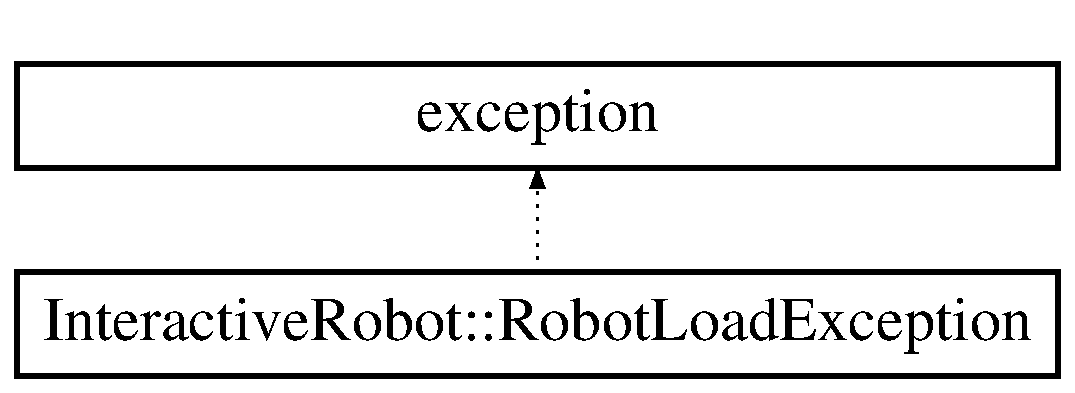
\includegraphics[height=2.000000cm]{class_interactive_robot_1_1_robot_load_exception}
\end{center}
\end{figure}


\subsection{Detailed Description}
exception thrown when a problem occurs 

The documentation for this class was generated from the following file\-:\begin{DoxyCompactItemize}
\item 
doc/pr2\-\_\-tutorials/interactivity/src/interactive\-\_\-robot.\-h\end{DoxyCompactItemize}

\section{tutorialformatter.\-Tutorial\-Formatter\-Directive Class Reference}
\label{classtutorialformatter_1_1_tutorial_formatter_directive}\index{tutorialformatter.\-Tutorial\-Formatter\-Directive@{tutorialformatter.\-Tutorial\-Formatter\-Directive}}
Inheritance diagram for tutorialformatter.\-Tutorial\-Formatter\-Directive\-:\begin{figure}[H]
\begin{center}
\leavevmode
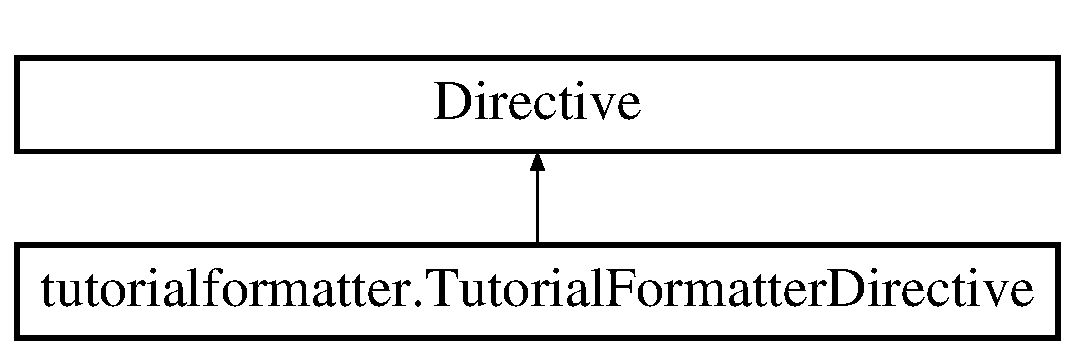
\includegraphics[height=2.000000cm]{classtutorialformatter_1_1_tutorial_formatter_directive}
\end{center}
\end{figure}
\subsection*{Public Member Functions}
\begin{DoxyCompactItemize}
\item 
def {\bfseries flatten\-\_\-sub\-\_\-tutorials}\label{classtutorialformatter_1_1_tutorial_formatter_directive_acfbe455cba049bf6073d93d1d99343b5}

\item 
def {\bfseries run}\label{classtutorialformatter_1_1_tutorial_formatter_directive_aae41fdd749ed9e30ac1c0a36112db384}

\end{DoxyCompactItemize}
\subsection*{Static Public Attributes}
\begin{DoxyCompactItemize}
\item 
{\bfseries has\-\_\-content} = False\label{classtutorialformatter_1_1_tutorial_formatter_directive_af0c47bdd1efa8de261098e93f90555b1}

\item 
{\bfseries final\-\_\-argument\-\_\-whitespace} = True\label{classtutorialformatter_1_1_tutorial_formatter_directive_af84e86e38bf4983b5a628d183899942b}

\item 
int {\bfseries required\-\_\-arguments} = 1\label{classtutorialformatter_1_1_tutorial_formatter_directive_ac578c9b7e68dd4d8bfc3363c3cbff6db}

\item 
tuple {\bfseries option\-\_\-spec}
\end{DoxyCompactItemize}


\subsection{Member Data Documentation}
\index{tutorialformatter\-::\-Tutorial\-Formatter\-Directive@{tutorialformatter\-::\-Tutorial\-Formatter\-Directive}!option\-\_\-spec@{option\-\_\-spec}}
\index{option\-\_\-spec@{option\-\_\-spec}!tutorialformatter::TutorialFormatterDirective@{tutorialformatter\-::\-Tutorial\-Formatter\-Directive}}
\subsubsection[{option\-\_\-spec}]{\setlength{\rightskip}{0pt plus 5cm}tuple tutorialformatter.\-Tutorial\-Formatter\-Directive.\-option\-\_\-spec\hspace{0.3cm}{\ttfamily [static]}}\label{classtutorialformatter_1_1_tutorial_formatter_directive_a7bbf9985e8df9db8766f93b4ed82f4c4}
{\bfseries Initial value\-:}
\begin{DoxyCode}
1 = dict(shell=flag, prompt=flag, nostderr=flag,
2                        in\_srcdir=flag, extraargs=unchanged,
3                        until=unchanged)
\end{DoxyCode}


The documentation for this class was generated from the following file\-:\begin{DoxyCompactItemize}
\item 
\-\_\-scripts/tutorialformatter.\-py\end{DoxyCompactItemize}

%--- End generated contents ---

% Index
\newpage
\phantomsection
\addcontentsline{toc}{chapter}{Index}
\printindex

\end{document}
